\ylDisplay{Paadid} % Ülesande nimi
{Tundmatu autor} % Autor
{lõppvoor} % Voor
{2013} % Aasta
{P 10} % Ülesande nr.
{3} % Raskustase
{
% Teema: Mehaanika

\ifStatement
 Laial jõel sõidavad kaks paati, mõlema kiirused ja kiiruste suunad on konstantsed. Veevoolu kiirus on jões samuti kõikjal üks ja sama ning paralleelne kallastega. Juuresolev foto on tehtud õhust, otse ülevalt alla; paatide asukohad on tähistatud ruudu ja kolmnurgaga, paatidelt vette kukkunud praht aga tähekestega. Üks paat alustas teekonda punktist $A$; on teada, et paadid kohtusid. Milisest jõekalda punktist alustas teekonda teine paat? Lahendus leidke geomeetrilise konstrueerimise teel lisalehel.
\begin{center}
	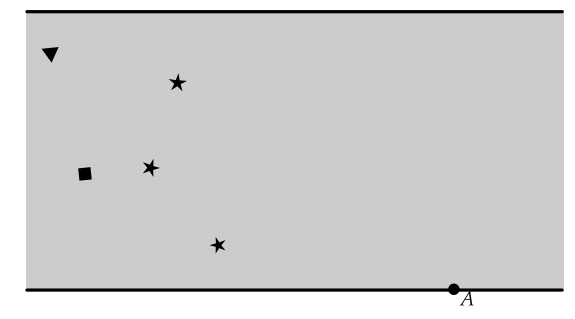
\includegraphics[width=0.5\linewidth]{2013-v3p-10-yl.PNG}
\end{center}
\fi

\ifHint
Kolmnurkne paat on kahe prugiga ühel joonel, seetõttu pidid need sellest paadist olema kukkunud.
\fi

\ifSolution
Leiame paatide trajektoorid veega seotud taustsüsteemis — need on sinised jooned joonisel (kolmnurkne paat on kahe prugiga ühel joonel, seetõttu pidid need sellest paadist olema kukkunud). Laevad kohtusid siniste joonte lõikepunktis. Kolmnurkse laeva trajektoor maaga seotud taustsüsteemis läheb läbi punkti $A$ (punane joon). Laevade kohtumispunkt maaga seotud taustsüsteemis peab olema samuti punasel joonel ning siniste joonte lõikepunktiga samal kõrgusel (lillal joonel). Ühendades lilla ja punase joone lõikepunkti teise paadi asukohaga leiame teise paadi trajektoori maaga seotud taustsüsteemis ning selle lähtepunkti $B$.
\begin{center}
	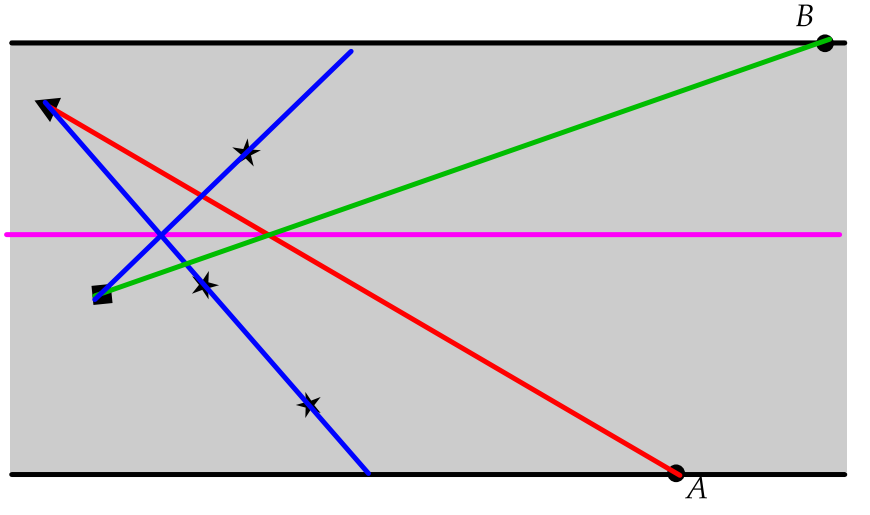
\includegraphics[width=0.5\linewidth]{2013-v3p-10-lah.PNG}
\end{center}
\fi
}
